\documentclass[letterpaper,10pt,serif,draftclsnofoot,onecolumn,compsoc,titlepage]{IEEEtran}

\usepackage{graphicx}                                        
\usepackage{amssymb}                                         
\usepackage{amsmath}                                         
\usepackage{amsthm}                                          
\usepackage{cite}
\usepackage{alltt}                                           
\usepackage{float}
\usepackage{color}
\usepackage[hyphens]{url}
\usepackage{pgfgantt}
\usepackage{rotating}
\usepackage{enumitem}
\usepackage{gensymb}
\usepackage[T1]{fontenc}

\usepackage{balance}
\usepackage[TABBOTCAP, tight]{subfigure}
\usepackage{enumitem}

\usepackage{geometry}
\geometry{margin=.75in}
\usepackage{hyperref}
\usepackage{breakurl}
%\usetikzlibrary{shapes, positioning, calc}
\usepackage{caption}
\usepackage{listings}
%\usepackage[utf8]{inputenc}
%pull in the necessary preamble matter for pygments output

\usepackage{listings}
\definecolor{dkgreen}{rgb}{0,0.6,0}
\definecolor{gray}{rgb}{0.5,0.5,0.5}
\definecolor{mauve}{rgb}{0.58,0,0.82}

\lstset{frame=tb,
  %language=Java,
  aboveskip=3mm,
  belowskip=3mm,
  showstringspaces=false,
  columns=flexible,
  basicstyle={\small\ttfamily},
  numbers=none,
  %numberstyle=\tiny\color{gray},
  %keywordstyle=\color{blue},
  %commentstyle=\color{dkgreen},
  %stringstyle=\color{mauve},
  breaklines=true,
  breakatwhitespace=true,
  tabsize=3
}

%% The following metadata will show up in the PDF properties
\hypersetup{
   colorlinks = true,
   citecolor = black,
   linkcolor = black,
   urlcolor = black,
   breaklinks = true,
   pdfauthor = {Shu-Ping Chien, Brock Smedley, W Keith Striby Jr},
   pdfkeywords = {CS463 "Senior Project" Final Report},
   pdftitle = {CS463 Final Report},
   pdfsubject = {CS463 Final Report},
   pdfpagemode = UseNone
}

\parindent = 0.0 in
\parskip = 0.1 in
\title{Final Report: Multi-Camera, SoM Based, Real-Time Video Processing for UAS and VR/AR Applications}
\author{Area 51: Shu-Ping Chien, Brock Smedley, W Keith Striby Jr \\ 12 June 2018 \\ CS463, Senior Software Engineering Project, Spring 2018}


\begin{document}
\begin{titlepage}
\maketitle

\begin{abstract}

Write me \\


\thispagestyle{empty}
\end{abstract}
\end{titlepage}

\newpage
\tableofcontents

\newpage

\section{Project Introduction}

\subsection{Problem}
% talk about 1) what's being requested, 2) who requested it & why, & its importance
% 2-3 paragraphs, minimum

\subsection{Persons Involved and Their Role}
% talk about: 1) members of the team, roles, restate client & state his role

\newpage 

\section{Requirements Document}

\section{Introduction}

\subsection{Purpose}

This software requirements specification is intended to define the requirements of the 
project for developing a multi-camera, multispectral image processing system, that 
operates on an SoM at near real-time, for use in air based 
applications. Defined requirements will allow for a contract between us, the 
developers, and Rockwell Collins, our client, on what Rockwell Collins wants us to 
deliver in their desired software. This document is intended for review and reference 
by both the developers and the clients.\\

\subsection{Scope}

The product outlined in this requirements document will be the multi-camera, SoM based,
 near real-time video processing for UAS and VR/AR applications. This product will need to 
 be able to generate a stitched video output from a multi-camera input. The product is 
 intended to help initialize our client's development of a cheaper alternative to a 
 product that is currently offered to their customers.\\

The software products that will be produced include software for a stitched video output 
from the NVIDIA TX1/2, receiving the input from two visible band cameras. 
The video output is expected to be near real-time, and the latency from the camera 
input to the video output is expected to be improved upon throughout the project. Video 
output stretch goals are to have software that fuses the video output from the input of 
three, four, five, and six cameras; and to have up to four infrared band inputs.\\

Output display stretch goals will be to incorporate IMU data, orientation tracking 
data, GPS data, and geolocate imagery. Two final stretch goals are packaging the 
hardware for flight, and interfacing the system to support the client's desired 
cameras for input.\\

The goal of the software is to contribute to a project that will assist pilots during 
low visibility conditions during the day, night, and inclement weather for all phases 
of flight. The video input from infrared and visible band cameras combined with 
on-board sensor input, and databases will enhance a pilot's vision for a UAS.\\

\subsection{Definitions, Acronyms, Abbreviations}

\subsubsection{Definitions}

\begin{tabular}{|l|p{11cm}|}
	\hline
	\textbf{Term} & \textbf{Definition}\\
	\hline
	geolocate imagery & image with associated location information.\\
	\hline
	low visibility & Inability to see clearly with the naked eye.\\
	\hline	
	multiple cameras & At least two cameras, but a maximum of six cameras for 
	video input.\\
	\hline
	near real-time & Fast enough that a human could not notice the time 
	delay (lag) between \newline real life images and images displayed by the system.\\
	\hline
	NVIDIA TX1/2 & NVIDIA GPUs, the Jetson TX1 or the Jetson TX2.\\
	\hline
	spectral bands & Electromagnetic frequency ranges; different 
	spectrums of light, including \newline but not limited to infrared 
	and visible light.\\
	\hline
	standalone & The system performs its functionality independent of another
	system, in our product's case it will be independent of a development kit. \\
	\hline
	stitched (video) output & a composite image formed from multiple images\\
	\hline
	time division multiplexing & The illusion of simultaneous execution in a CPU due
	to a CPU being capable of running one process at a time.\\
	\hline
\end{tabular}

\subsubsection{Acronyms}

\begin{tabular}{|l|l|}
	\hline
	\textbf{Acronym} & \textbf{Term}\\
	\hline
	AR & Augmented Reality\\
	\hline
	CPU & Central Processing Unit\\
	\hline
	CSI & Camera Serial Interface\\
	\hline
	EVS & Enhanced Vision System\\
	\hline
	fps & Frames per second\\
	\hline
	GPS & Global Positioning System\\
	\hline
	GPU & Graphic Processing Unit\\
	\hline
	ISP & Image Signal Processors\\
	\hline
	IMU & Inertial Measurement Unit\\
	\hline
	HUD & Head-up Display\\
	\hline
	SoC & System-on-chip\\
	\hline
	SoM & System-on-module\\
	\hline
	SWaP-C & Size, weight, power and cost\\
	\hline
	UAS & Unmanned Aircraft System\\
	\hline
	VI & Video Input\\
	\hline
	VR & Virtual Reality\\
	\hline
\end{tabular}

\subsection{Overview}

This project aims to create a product that is capable of combining the video input from 
two or more cameras and produce an output at near real-time. Our proposed solution 
will use an NVIDIA Jetson TX1/2, which we will use for its integrated GPU and CPU.\\

We need this GPU to combine the images from multiple cameras. The end goal is to have 
a system that uses the input from multiple cameras that operate on the infrared and 
visible light spectral bands. By using these spectral bands, we should be able to 
produce an image that can be used to see in low-visibility situations, such as landing 
a UAS in fog.\\

The images we produce will be 2D representations of our collective image captures. In 
other words, we do not aim to create a 3D image or a dynamic focus image. This is 
certainly possible when using multiple cameras, but we simply aim to use multiple 
cameras on different spectral bands to create one image of one subject that is the 
combination of all images captured by the cameras.\\


\section{Overall Description}

\subsection{Product Perspective}

The system will be self-contained and consists of three parts: one NVIDIA TX1/2, 
one carrier board, and at least two cameras. The cameras connect to the carrier board, 
which is connected to the NVIDIA TX1/2. The NVIDIA TX1/2 is responsible for decoding 
the serial data retrieved by the CSI board from the cameras, and is then be used to 
execute the software for image processing and combining images from multiple cameras.\\

\begin{figure}[H]
	\centering
	\label{fig:ProductBlockDiagram}
	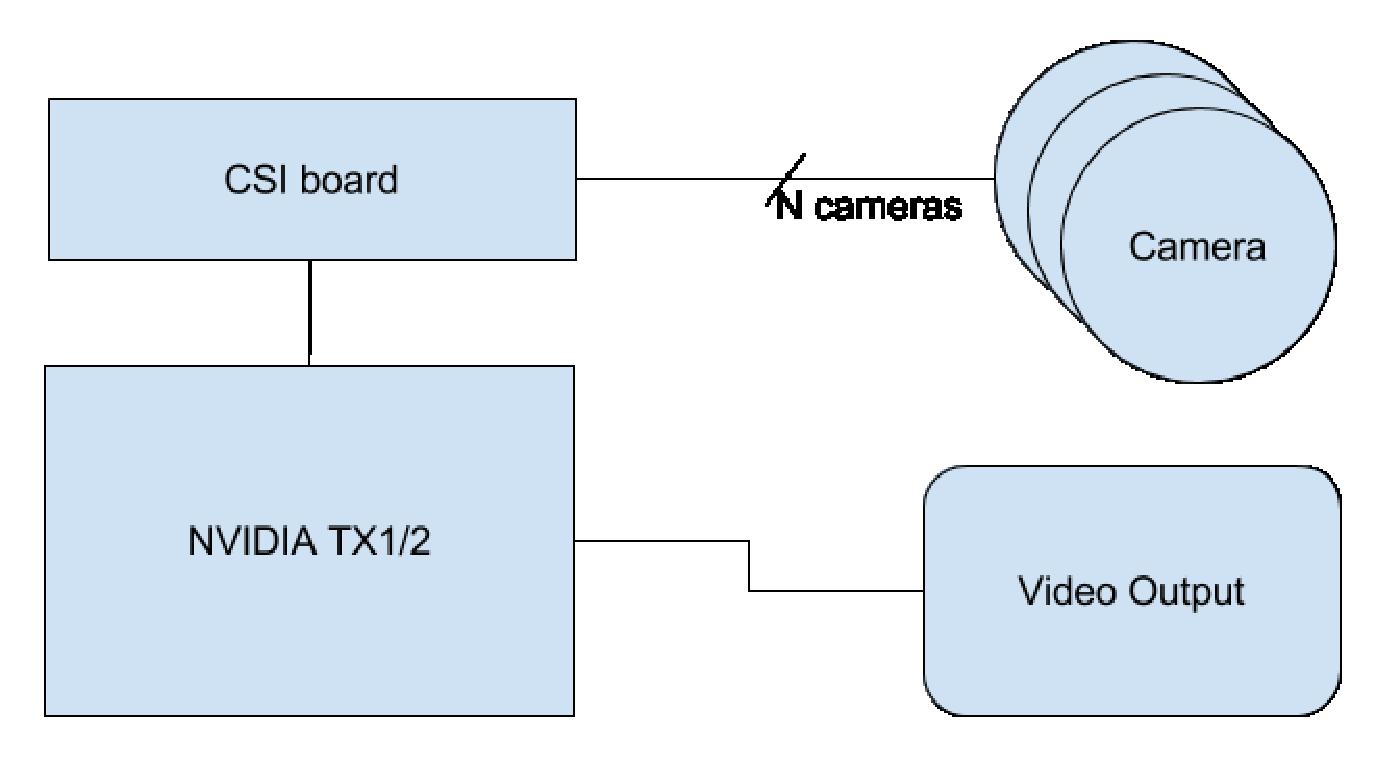
\includegraphics[width=10cm]{images/diagram.eps}
	\caption{Product Block Diagram \label{overflow}}
\end{figure}

\subsection{Product Functions}

The basic functionality of the product will be to produce stitched images on a video 
output that is provided by multiple camera inputs capable of sensing visible and 
infrared spectral bands. These images will be relayed in near real-time so that it 
can be used as a video feed for the pilot of a UAS during low visibility flight 
conditions. \\

A functional stretch goal for video output provided by camera input is to fuse the 
input from the visible and infrared spectral bands, which will overlay the two types of output 
and enhance the vision for a UAS pilot. \\

Output display functional stretch goals will be to provide indications from IMU data, 
orientation tracking data, GPS data, and geolocate imagery and have them displayed 
with the video output provided by the camera input. \\

\subsection{Constraints}

The client requires that the product's SoM be an NVIDIA TX1/2 to utilize its GPU 
and CSI ports. Due this product's application being on a UAS, its hardware must be 
compact to meet SWaP-C requirements set by the client. The system must be standalone 
and not rely on cloud computing and external databases. \\

The system must operate in near real-time, and therefore the video/camera feed(s) must be 
processed quickly enough for the user to be able to make snap decisions based on the feed. The 
NVIDIA TX1/2 should process each frame before the next one arrives to be processed. 
For example, when recording at 30 fps each output frame should be processed in 
less than 1/30 of a second.\\

\subsection{Assumptions \& Dependencies}

Software will be implemented on an NVIDIA TX1/2, and will be deployed with NVIDIA 
Jetpack software running on an Ubuntu machine. The NVIDIA TX1/2 is assumed to be 
capable of processing the data feed through its CSI interface. \\

Adequate power supplies are required; they should meet the NVIDIA TX1/2 system 
requirements. \\

All cameras in use should be aimed at same subject, capturing approximately the same 
image. Each camera should work independently of the system; if one fails, the others 
will still operate.\\

\section{Specific Requirements}

\subsection{Hardware Specifications}

\subsubsection{NVIDIA Jetson TX1/2}

\begin{enumerate}[label=\alph*]
	\item The NVIDIA TX1/2 will receive image data through its CSI interface from
	the carrier board, and process this data to produce a video output. The carrier
	board is providing input to the NVIDIA TX1/2 from multiple cameras. \\
	\item The development environment of NVIDIA TX1/2 is available on the Ubuntu 
	operating system, and the module supports software for image processing.\\ 
	\end{enumerate}

\subsubsection{Carrier Board}

\begin{enumerate}[label=\alph*]
	\item The carrier board should contain a CSI interface, which is used to transfer the
	input from up to six cameras to the NVIDIA TX1/2. \\
	\item The carrier board will provide output for a computer with data and signals that 
	can be used for subsequent image processing.\\
	\item The carrier board will be compatible with the NVIDIA TX1/2.\\
\end{enumerate}

\subsubsection{Cameras}

\begin{enumerate}[label=\alph*]
	\item Cameras that use the CSI interface are required in order to transfer image data to 
	the NVIDIA TX1/2.\\
	\item The transfer rate is expected to operate at near real-time, and the output format 
	from the cameras will be accepted by NVIDIA TX1/2.\\
	\item The cameras should be able to capture images from different spectral bands 
	which includes infrared and visible light.\\
	\item The quality of the camera is not a primary concern for our project, and its 
	function is to is provide input to the NVIDIA TX1/2 for testing video output. 
	A stretch goal involves providing an interface to accomodate for cameras that 
	produces a higher quality input, but the hardware to connect these cameras to the 
	carrier board does not appear to exist at this time.\\
\end{enumerate}

\subsection{Software Specifications}

\begin{enumerate}[label=\alph*]
	\item The software running on the TX1/2 should be able to decode the data streams 
	from each camera and provide a stitched video output.\\
	\item The software should be able to stitch images from infrared 
	and visible light spectral bands to produce a 2D video output. \\
	\item Latency of the data-processing in the software is expected to be near 
	real-time, therefore the programming implemented will be required to use either time
	division multiplexing or parallel processing. \\
	\item The software stretch goals are to:
	\begin{enumerate}
	 	\item Output a dual stitched video combined with a fused six-camera input.\\
		\item Incorporate IMU data, orientation tracking data, GPS data, and geolocate 
		imagery into the video output. An IMU is used to track linear and angular 
		motion of an object by using gyroscopes and accelerometers. Orientation 
		tracking utilizes sensor input to provide rotational and position data.\\
		\item Provide an interface to accomodate for cameras the meet quality
		requirements for video output. \\
	\end{enumerate} 
\end{enumerate}

\section{Development Schedule}
	\begin{ganttchart}
    	[hgrid, x unit=0.77mm, y unit chart=9.0mm, title label font=\normalsize, time slot format=isodate]
    	{2017-11-01}{2018-05-31}
    	\gantttitlecalendar{year, month=name}\\
    	\ganttbar{Task 1}{2017-11-01}{2017-11-30}\\
    	\ganttbar{Task 2}{2017-11-15}{2018-01-06}\\
    	\ganttbar{Task 3}{2018-01-01}{2018-01-31}\\
    	\ganttbar{Task 4}{2018-01-15}{2018-02-28}\\
    	\ganttbar{Task 5}{2018-03-01}{2018-03-31}\\
    	\ganttbar{Task 6}{2018-04-01}{2018-04-30}\\
    	\ganttbar{Task 7}{2018-05-01}{2018-05-31}\\
    	\ganttlink{elem0}{elem1}
    	\ganttlink{elem1}{elem2}
    	\ganttlink{elem2}{elem3}
	\end{ganttchart}
\begin{center}
	Fig. 2: Project Schedule
\end{center}	

\subsection{Development Schedule Tasks}
Task 1: Have hardware procured and assembled when received.\\
Task 2: Produce stitched video output from the input of two and three cameras, 
and have latency estimates produced.\\
Task 3: Produce a tiled video output from the input of six cameras.\\
Task 4: Produce a dual stitched video output that is combined into a fused 
six-camera output (stretch goal).\\
Task 5: Incorporate IMU data, orientation tracking data, GPS data, and 
geolocate imagery into the video output (stretch goals).\\
Task 6: Package the system hardware for flight (stretch goal).\\
Task 7: Produce a software interface for the system to accomodate higher 
quality cameras (stretch goal).\\

\section{Final Gantt Chart}
% record of what happened

\newpage 

\section{Design Document}
\section{Frontispiece}

\subsection{Date of issue and status}

01 December 2017, In-progress \\

\subsection{Issuing Organization}

Rockwell Collins, CS Capstone Group 51, Oregon State University \\

\subsection{Authorship}

Shu-Ping Chien, Brock Smedley, W Keith Stirby Jr \\

\section{Introduction}

\subsection{Purpose}

This document is a general description of design concepts that will be used for our 
multi-camera, SoM based, real-time video processing for UAS and VR/AR applications. 
It is a reference to guide the development of our product.  \\

\subsection{Scope}

Our product will receive input from multiple cameras and then provide a video output at 
near real-time. Our software will receive the pixel data from the cameras and format 
the pixel streams so that image processing can occur. Image processing will then stitch 
the multiple streams of pixels being received to create a combined output. The software 
will be flashed onto the NVIDIA TX1/2, which receives input from the carrier 
board that is connected to the cameras. \\

\subsection{Overview}

The development and design of our product requires: hardware interface and system 
architecture, receiving camera input and formatting for image processing, and image 
processing for video output. The structure of our document reflects these three areas 
of our software required for our product. \\ 

\newpage
\section{References}

\bibliographystyle{ieeetr}
\bibliography{SDD_Group51}

\subsection{Definitions, Acronyms, Abbreviations}

\subsubsection{Definitions}

\begin{tabular}{|l|p{11cm}|}
	\hline
	\textbf{Term} & \textbf{Definition}\\
	\hline
	multiple cameras & At least two cameras, but a maximum of six cameras for 
	video input.\\
	\hline
	near real-time & Fast enough that a human could not notice the time 
	delay (lag) between \newline real life images and images displayed by the system.\\
	\hline
	(NVIDIA) TX1/2 & NVIDIA GPUs, the Jetson TX1 or the Jetson TX2.\\
	\hline
	GitHub repository & version control software for source code hosting and development\\
	\hline
	spectral bands & Electromagnetic frequency ranges; different 
	spectrums of light, including \newline but not limited to infrared 
	and visible light.\\
	\hline
	stitch(ed) (video) output & a composite image formed from multiple images\\
	\hline
\end{tabular}

\subsubsection{Acronyms}

\begin{tabular}{|l|l|}
	\hline
	\textbf{Acronym} & \textbf{Term}\\
	\hline
	CSI & Camera Serial Interface\\
	\hline
	GPIO & General-purpose Input/Output\\
	\hline
	GPU & Graphic Processing Unit\\
	\hline
	I2C & The Inter-integrated Circuit Protocol\\
	\hline
	ISP & Image Signal Processors\\
	\hline
	L4T & Linux for Tegra \\
	\hline
	SoM & System-on-module\\
	\hline
	USB & Universal Serial Bus\\
	\hline
	V4L2 & Video for Linux 2 \\
	\hline
	VI & Video Input\\
	\hline
\end{tabular}

\newpage
\section{System Overview}  

\subsection{Identified Stakeholders and Design Concerns}

Rockwell Collins is the primary customer of this product. The company provides 
engineering products in the aviation industry for commercial and military customers. 
Rockwell Collins is the primary user of the product and it is contributing 
to the development of a system that will be used in UAS and VR/AR applications. \\

\subsection{Hardware Context}

The hardware used in our product will be the NVIDIA Jetson TX1/2 as our SoM, 
a carrier board, and cameras. The input from cameras will be transferred through 
carrier boards, and the TX1/2 will format and process the input to produce a 
video output. The software we're developing will be on the TX1/2. \\

\subsection{Software Context}

The software pieces in this project include: GStreamer for transforming video input 
from CSI for image processing, and OpenGL development environment for image processing 
to produce the video output. The pipeline feature in GStreamer will reduce 
cost on time and storage to help achieve near real-time image processing. The OpenGL 
will stitch input images from GStreamer and print the output to the display device. \\

\section{System Architecture}

\subsection{Interfaces}

The NVIDIA TX1/2 is an SoM with an ARM processor and an NVIDIA GPU. It includes several 
interfaces that can be used to exchange data with the module such as Ethernet, USB, 
I2C, and GPIO, among others. These connect to the TX1/2 via a 400-pin connector that 
attaches to a carrier board, which has a set of ports to interface with. These 
interfaces will be used in our implementation of the project for varying purposes. \\

\subsubsection{Ethernet}

Ethernet is essential for development. It will allow us to connect to the internet and 
will also allow us to control the system remotely using SSH. Ethernet will likely not 
be used in the final implementation, however. The final implementation will likely 
have an image flashed directly to its memory so that there is no need to download any 
new software or data. The carrier board we will be using in the final implementation 
may not have an Ethernet connection, but if it does not have it, we can attach the TX1/2 
to the dev board that it came with, which has at least one connection for every 
interface that the TX1/2 supports. \\

\subsubsection{USB}

USB will be necessary for flashing the TX1/2 with a new image. This only needs to be 
done once at the start of development, and possibly again when a production image is 
ready to be flashed, but it is nonetheless required for development. USB can also be 
used for simple file transfers in cases where the internet is not available. USB will 
also not be present on the final product, but it should not be necessary at that stage; 
we will not be using USB for any system-critical functions. The TX1/2 can always be 
plugged into the dev board if changes to the system need to be made, and then 
re-attached to the final-product board with the new data on it.\\

\subsubsection{I2C \& GPIO}

I2C and GPIO will be used in later phases of the project which we may not actually 
work on. These interfaces can be used for connecting things like environmental sensors 
and control interfaces like buttons and knobs. Our portion of the project will focus 
solely on creating the camera system on the TX1/2 which can then be expanded upon by 
other teams. \\

\subsection{Architecture}

\subsubsection{Operating Systems}

The TX1/2 supports ARM Linux 4 operating systems, and the OS we will be using for this 
project is L4T. L4T is an ubuntu variant that comes preloaded with a 
bundle of software that can be used to take advantage of the processing power that 
the TX1/2 has to offer. L4T is simply an Ubuntu ARM image with NVIDIA drivers 
pre-installed. Using L4T takes the guesswork out of developing the software 
environment so that more time can be spent developing the core solution. \\

\subsubsection{Deployment Software}

L4T will be flashed onto the TX1/2 system memory using NVIDIA Jetpack. Jetpack allows 
us to choose the operating system and software to be installed on the TX1/2. It runs on 
a separate Ubuntu host which is connected to the TX1/2 via USB and a router connecting 
both the machines to the internet, and can be downloaded from the NVIDIA's website 
after creating an account. Ubuntu is not required to run Jetpack, but NVIDIA strongly 
recommends it, and Ubuntu is a very user-friendly and robust operating system, so it 
will suit our development needs perfectly. \\

\subsubsection{Development}

Once L4T is flashed to the TX1/2 from Jetpack, we can use the TX1/2 like a normal 
computer, using USB to connect a mouse \& keyboard, and HDMI to connect a monitor. 
Development can occur directly on the TX1/2 or remotely via SSH (Ethernet). We will 
likely use a combination of the two; sometimes it is required, for example when 
internet access is not available; sometimes it is more convenient. \\

We will also make use of a GitHub repository to keep our code, which can be accessed 
by the TX1/2 via the internet. This will allow each group member to work on different 
parts of the project simultaneously without interfering with other group members' 
work. Most Linux variants come with a version of Git, but if L4T does not, then we 
can always install it using Ubuntu's package manager. \\

\subsection{Making Camera Input Ready for Image Processing}

\subsubsection{Multimedia API}

The raw pixel data from the cameras will be sent through the CSI and must be converted 
to the BRG color space in the VI unit before being sent to the ISPs. 
Application development can use either libargus API 
included in L4T or GStreamer plugin to prepare the raw pixel data in the VI unit, and 
therefore convert the data to a format that is recognizable by the ISP. NVIDIA does not 
support V4L2 when using CSI cameras, but GStreamer does and therefore will be used in 
our software.  \\

	\begin{figure}[H]
		\centering
		\label{fig:MultimediaBlockDiagram}
		\includegraphics[width=10cm]{images/multimedia-block.eps}
		\caption{Jetson TX1/2 Camera Subsystem\cite{CSubDia} \label{overflow}}
	\end{figure}

\subsubsection{GStreamer}

GStreamer architecture utilizes pipelines to process media and connect the processing 
elements. An additional architecture GStreamer uses is plugin, which provides each 
processing element. \\

\paragraph{Installing GStreamer}\mbox{} \\ 

To install GStreamer 1.0 and plugins the following commands will be entered in the 
command line in order\cite{GStmUG}: \\

	\begin{enumerate}
		\item\texttt{\$ sudo add-apt-repository universe} \\
		\item\texttt{\$ sudo add-apt-repository multiverse} \\
		\item\texttt{\$ sudo apt-get update} \\
		\item\texttt{\$ sudo apt-get install gstreamer1.0-tools gstreamer1.0-alsa 
			gstreamer1.0-plugins-base \newline gstreamer1.0-plugins-good 
			gstreamer1.0-plugins-bad gstreamer1.0-plugins-ugly \newline
			gstreamer1.0-libav} \\
		\item\texttt{\$ sudo apt-get install libgstreamer1.0-dev libgstreamer-plugins-base1.0-dev \newline
		libgstreamer-plugins-good1.0-dev libgstreamer-plugins-bad1.0-dev} \\
	\end{enumerate}

\paragraph{GStreamer Plugins}\mbox{} \\ 

To display what a camera is capturing \texttt{nvcamerasrc} included in the piping, 
and is a plugin that allows options for our software to control ISP properties. \\

For converting video frames from the CSI camera the \texttt{videoconvert} plugin will 
be included in piping, along with \texttt{video/x-raw, format=(string){}} to specify 
details on the conversion input and output. \\

\subsection{Image Processing for Video Output}

Since the  NVIDIA Jetpack includes OpenGL 4.3, 4.4, and 4.5, the program will use 
OpenGL and the OpenGL Shading Language for image processing to detect edge and draw on 
images, and the output will be sent to a display device. \\

\subsubsection{OpenGL Environment Setup}

Before drawing anything with OpenGL, the OpenGL environment need to be set up at first 
in order to specify the size of screen window and viewing features. Then the output 
images will be generated in display function, where the program does image processing 
and draws to. \\

\subsubsection{Bind Video Input as Textures}

The video output will be read as textures and processed in the shaders. The OpenGL 
binds a texture with the following code:\\

\begin{tabular}{|p{15cm}|}
	\begin{lstlisting}
		GLuint tex;
		glGenTextures(1, &tex);
		glBindTexture(GL_TEXTURE_2D, tex);
		glTexParameteri(GL_TEXTURE_2D, GL_TEXTURE_WRAP_S, GL_REPEAT);
		glTexParameteri(GL_TEXTURE_2D, GL_TEXTURE_WRAP_T,GL_REPEAT);
		glTexParameteri(GL_TEXTURE_2D, GL_TEXTURE_MIN_FILTER, GL_LINEAR);
		glTexParameteri(GL_TEXTURE_2D, GL_TEXTURE_MAG_FILTER, GL_LINEAR);
		glTexImage2D(GL_TEXTURE_2D, 0, GL_RGB, width, height, 0, GL_RGB, GL_UNSIGNED_BYTE, image);
	\end{lstlisting}
\end{tabular}

Where the image is the a loaded texture image from video output, and it is composed of 
2D arrays of pixels. Then the texture can be used in the OpenGL Shading Language with 
the created shaders.\\

There are two shaders used in this project, vertex shader and fragment shader. The 
vertex shader needs to be modified so that the texture coordinates can be interpolated 
over the fragments, and with the output from the vertex shader, the fragment shader 
fused images as output. \\

\subsubsection{Vertex Shader}

Since textures are sampled using texture coordinates, which are represented as s and 
t, the vertex shader uses the input to modify the texture coordinates and pass to 
fragment shader as output. In order to provide access to the texture in the fragment 
shader, the program will set the texture as uniform variable of type sampler2D in the 
fragment shader.\\

\subsubsection{Fragment Shader}

The fragment shader renders an image by filling color in pixels. The color filled in a 
pixel will be determined based on the texture, where the program read the RGB 
information with output of texture coordinate from vertex shader.\\

In OpenGL:\\
\begin{tabular}{|p{15cm}|}
	\begin{lstlisting}
		glUniform1i(glGetUniformLocation(shaderProgram, "texName"), 0);
	\end{lstlisting}
\end{tabular}
\\
\\
In Fragment Shader:\\
\begin{tabular}{|p{15cm}|}
	\begin{lstlisting}
   		in vec2 Texcoord;    //from vertex shader
   		out vec4 outColor;
   		uniform sampler2D texName;

   		void main()
   		{
        	outColor = texture(tex, Texcoord);
   		}
	\end{lstlisting}
\end{tabular}

In this code in the fragment shader, the output, outColor, will be the color from 
function texture(tex, Texcoord). By controlling the Texcoord, the fragment shader 
can draw on specific coordinate to generate an output image.\\

\newpage

\section{Technology Review}


\newpage

\section{Weekly Blog Posts}


\newpage

\section{Final Poster}


\newpage

\section{Project Documentation}


\newpage

\section{Recommended Technical Resources for Learning More}


\newpage

\section{Conclusions and Reflections}


\newpage

\section{Appendix 1: Essential Code Listings}
% doesn't have to be everything, but there should be stuff here for someone to learn from


\nocite{*}
\end{document}
